\section{Cloud Architecture and Design}

This system will be deployed using Infrastructure as a Service (IaaS) on Amazon Web Services (AWS).

\subsection{Platform Selection}



\subsection{Design Assumptions}

The preparation of this document makes a few key assumptions that will need to be confirmed with SmartV. These are the following: 

\begin{itemize}
    \item \textbf{Geographic Scope:}
    \item \textbf{Provision of Software:}
    \item \textbf{User Accounts:}
\end{itemize}

\subsection{Infrastructure Design}

\begin{figure}[H]\label{fig:awsdiagram}
    \centering
    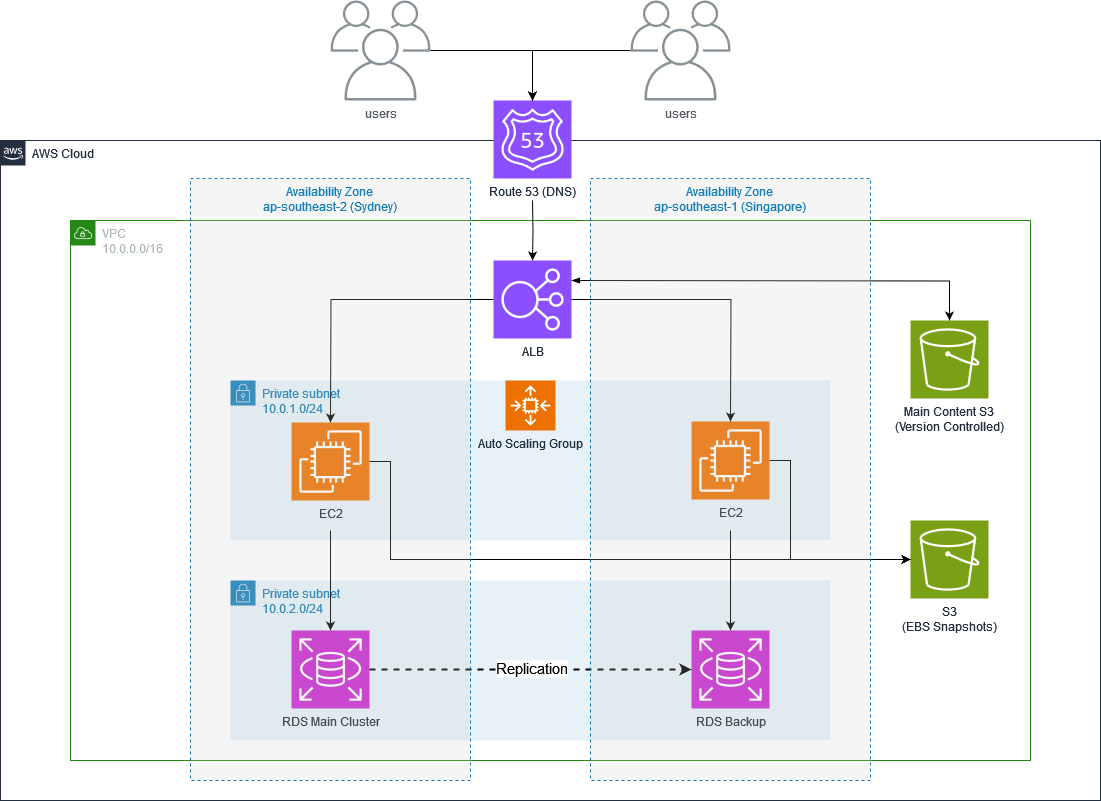
\includegraphics[width=\textwidth]{cci_aws}
    \caption{Cloud Infrastructure Topology}
\end{figure}

\subsection{Infrastructure Components}
\label{sec:infrastructure-components}

\subsubsection*{DNS (Route 53)}

Allowing global access through http, a DNS record is needed and will be achieved through an AWS Route 53 domain. This will transfer users to the ALB.

\subsubsection*{Network (ALB)}

To balance load across seperate compute clusters, an application load balancer (ALB) will handle distribution of incoming requests to allow transparent scaling of compute abstracted from the user, meaning bucekts of storage can scale infinitely.

\subsubsection*{Compute (EC2)}

Using an autoscaling group of EC2 instances of type ``p3.8xlarge'', compute will be handled and scaled with demand. The instance types are very large to accomodate for the intense RAM, CPU, and GPU requirements video demands. A key feature of S3 is the inherent scalability, as this is abstracted away from the end user. The use of this instance scale also allows networking performance of 10 Gbps. This will be very helpful as the most intense network requirements are occurring internally on AWS, between compute and content storage on S3.

\subsubsection*{Content Storage (S3)}

AWS Simple Storage Service (S3) allows for cheap and easy object storage through a HTTP API endpoint. This is suitable for storing the large files used by the service, and allowing avilability across the platform.

\subsubsection*{Backup Storage (S3)}

Snapshots of the drives associated with compute instances, the elastic block storage (EBS) drives, will be palced daily in a seperate S3 bucket to allow disaster recovery of user's work and files retained locally on the compute instance.

\subsubsection*{User Database (RDS)}

AWS Relational Database System (RDS) will be used to handle user information such as login, account details, and payment information. Using a traditional database system is suitable over S3 as it allows structure and replication.

\subsubsection*{Network (Public)}

The entire cloud system will exist within a private VPC, with the only publically exposed element being the ALB accessible through the Route 53 DNS record or associated IP address.

\subsubsection*{Network (Internal)}

Internally, the platform is networked through a private IPv4 subnet in CIDR block 10.0.0.0/16. Each private subnet in turn has it's own CIDR block with a netmask of 24. Compute and the RDS service reside in seperate private subnets to improve security.

\subsubsection*{Scaling (Compute)}

Using EC2 autoscaling groups, AWS will launch new compute instances as demand increases on pre-existing ones, placing them behind the ALB. Retaining a minimum of 1 instance ensures constant availability. An option available is keep ``warm pools'' of compute instances pre-initialized but not in use, allowing near instant upscaling as demand spikes.

\subsubsection*{High Availability}

High availability will be achieved through seperating cloud resources across two AWS availability zones (AZs), allowing an entire region of AWS to lose access, while maintaining service for customers. It also allows upgrades to infrastructure and software to cause a temporary planned outage in one region while maintaining uninterrupted service globally.

\subsection{Pricing}

% https://calculator.aws/#/addService
